\section{Auswertung}
\label{sec:Auswertung}

\subsection{Untersuchung der Filterkurve}

Zunächst wird Durchlassfrequenz $\nu$ des Selektivverstärkers bestimmt. Die 
gemessenen Wertepaare von Frequenz $\nu$ und Spannung $U_\text{A}$ sind in 
Tabelle \ref{tab:Messdaten1} aufgeführt. 

\begin{table}
\centering
\caption{Messwerte der Filterkurve des Selektivverstärkers.}
\label{tab:Messdaten1}
\sisetup{table-format=2.1}
\begin{tabular}{c c}
\toprule
$\nu \,/\, \si{\kilo\hertz}$ & $U_\text{A} \,/\, \si{\volt}$\\
\midrule
0,00 & 100\\
\bottomrule
\end{tabular}
\end{table}

Die gemessene Frequenz $\nu$ wird gegen die Spannung $U_\text{A}$ aufgetragen. Das 
Ergebnis ist in Abbildung \ref{fig:plot1} zu finden. 

\begin{figure}
  \centering
  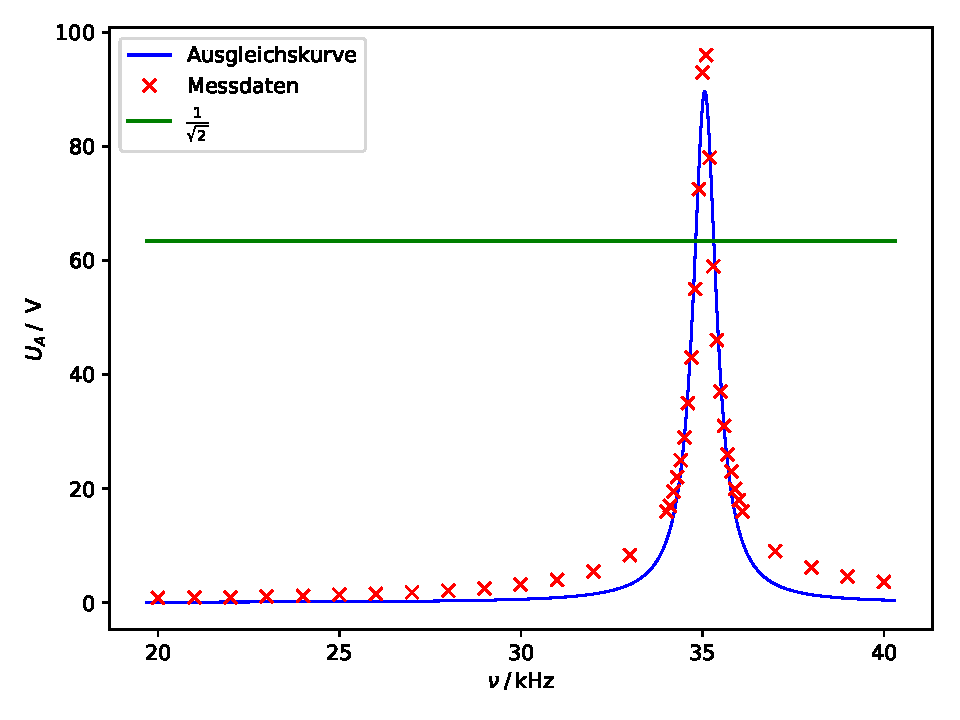
\includegraphics{content/plot1.pdf}
  \caption{Filterkurve des Selektivverstärkers.}
  \label{fig:plot1}
\end{figure}

Die Durchlassfrequenz ergibt sich demnach zu 

\begin{equation}
\nu _\text{A} = \SI{}{\kilo\hertz}.
\end{equation}

\subsection{Experimentelle Bestimmung der Suszeptibilität}

Die Messdaten zur Bestimmung der Suszeptibilität $\chi$ sind in Tabelle 
\ref{tab:Messdaten3}, \ref{tab:Messdaten4} und \ref{tab:Messdaten5} zu finden. 
Der Koeffizient Q muss dabei durch den Querschnitt

\begin{equation}
Q_\text{real} = \frac{m}{\rho \cdot l}
\end{equation}

ersetzt werden. Dieser ergibt sich durch die Länge $l$, die Masse $m$ und 
die Dichte $\rho$ der Probe. Diesen Querschnitt müsste die Probe haben, wenn 
sie aus einem Einkristall bestünde.

\begin{table}
\centering
\caption{$Q_\text{real}$ der verwendeten Stoffe.}
\label{tab:Messdaten2}
\sisetup{table-format=2.1}
\begin{tabular}{c c}
\toprule
Stoff & $Q_\text{real} \,/\, \si{\centi\meter²}$\\
\midrule
$Gd_2O_3$ & 100\\
$Dy_2O_3$ &\\
$Nd_2O_3$ &\\
\bottomrule
\end{tabular}
\end{table}

Es wurde mit der Eingangsspannung $U_\text{E} = \SI{1}{\volt}$ gemessen. Der 
Spulenquerschnitt ist mit $F = \SI{}{\meter²}$ gegeben. Aus den Messwerten 
können nun die Suszeptibilitäten $\chi$ berechnet werden, nach Bereinigung 
um die Verstärkung $V$. Diese finden sich in Tabelle \ref{tab:Messdaten3}, 
\ref{tab:Messdaten4} und \ref{tab:Messdaten5}.
Dabei bezeichnen $U_\text{m}$ und $R_\text{m}$ die Spannung und Widerstände, 
während die Probe sich in der Spule befindet. $U_\text{0}$ und $R_\text{0}$
sind entsprechend die Werte ohne Probe in der Spule. 

\begin{table}
\centering
\caption{Messwerten und Suszeptibilitäten für $Gd_2O_3$}
\label{tab:Messdaten3}
\sisetup{table-format=2.1}
\begin{tabular}{c c c c c c}
\toprule
$U_\text{m} \,/\, \si{\milli\volt}$ & $R_\text{m} \,/\, \si{\ohm}$ & $U_\text{0} \,/\, \si{\milli\volt}$& $R_\text{0} \,/\, \si{\ohm}$ & $\chi _\text{U}$ & $\chi _\text{R}$ \\
\midrule
0,00 & 100 & 4 & 5 & 6 & 7\\
\bottomrule
\end{tabular}
\end{table}

\begin{table}
\centering
\caption{Messwerten und Suszeptibilitäten für $Dy_2O_3$}
\label{tab:Messdaten4}
\sisetup{table-format=2.1}
\begin{tabular}{c c c c c c}
\toprule
$U_\text{m} \,/\, \si{\milli\volt}$ & $R_\text{m} \,/\, \si{\ohm}$ & $U_\text{0} \,/\, \si{\milli\volt}$& $R_\text{0} \,/\, \si{\ohm}$ & $\chi _\text{U}$ & $\chi _\text{R}$ \\
\midrule
0,00 & 100 & 4 & 5 & 6 & 7\\
\bottomrule
\end{tabular}
\end{table}

\begin{table}
\centering
\caption{Messwerten und Suszeptibilitäten für $Nd_2O_3$}
\label{tab:Messdaten5}
\sisetup{table-format=2.1}
\begin{tabular}{c c c c c c}
\toprule
$U_\text{m} \,/\, \si{\milli\volt}$ & $R_\text{m} \,/\, \si{\ohm}$ & $U_\text{0} \,/\, \si{\milli\volt}$& $R_\text{0} \,/\, \si{\ohm}$ & $\chi _\text{U}$ & $\chi _\text{R}$ \\
\midrule
0,00 & 100 & 4 & 5 & 6 & 7\\
\bottomrule
\end{tabular}
\end{table}

Aus den Suszeptibilitäten können nun die Mittelwerte berechnet werden, 
sodass sich Tabelle \ref{tab:Messdaten6} ergibt. 

\begin{table}
\centering
\caption{Berechnete Suszeptibilitäten.}
\label{tab:Messdaten6}
\sisetup{table-format=2.1}
\begin{tabular}{c c c c}
\toprule
& $Gd_2O_3$ & $Dy_2O_3$ & $Nd_2O_3$ \\
\midrule
$\chi_\text{theo}$ & 0,0138 & 0,0254 & 0,0030\\
$\chi_\text{U}$ & 100 & 4 & 5\\
$\chi_\text{R}$ & 100 & 4 & 5\\
\bottomrule
\end{tabular}
\end{table}

Damit ergeben sich die Abweichungen in Tabelle \ref{tab:Messdaten7} vom theoretischem 
Wert. 

\begin{table}
\centering
\caption{Abweichungen zum theoretischem Wert.}
\label{tab:Messdaten7}
\sisetup{table-format=2.1}
\begin{tabular}{c c c}
\toprule
& $\frac{\chi_\text{theo}-\chi_\text{U}}{\chi_\text{theo}}$ 
& $\frac{\chi_\text{theo}-\chi_\text{R}}{\chi_\text{theo}}$\\
\midrule
$Dy_2O_3$ & & \\
$Nd_2O_3$ & & \\
$Gd_2O_3$ & & \\
\bottomrule
\end{tabular}
\end{table}
